%%%%%%%%%%%%%%%%%%%%%%%%%%%%%%%%%%%%%%%%%%%%%%%%%%%%%%%
%% Bachelor's & Master's Thesis Template             %%
%% Copyleft by Artur M. Brodzki & Piotr Woźniak      %%
%% Faculty of Electronics and Information Technology %%
%% Warsaw University of Technology, 2019-2020        %%
%%%%%%%%%%%%%%%%%%%%%%%%%%%%%%%%%%%%%%%%%%%%%%%%%%%%%%%

\documentclass[
    left=2.5cm,         % Sadly, generic margin parameter
    right=2.5cm,        % doesnt't work, as it is
    top=2.5cm,          % superseded by more specific
    bottom=3cm,         % left...bottom parameters.
    bindingoffset=6mm,  % Optional binding offset.
    nohyphenation=false % You may turn off hyphenation, if don't like.
]{eiti/eiti-thesis}

\langpol % Dla języka angielskiego mamy \langeng
\graphicspath{{img/}}             % Katalog z obrazkami.
\addbibresource{bibliografia.bib} % Plik .bib z bibliografią

\begin{document}

%--------------------------------------
% Strona tytułowa
%--------------------------------------
\EngineerThesis % Dla pracy inżynierskiej mamy \EngineerThesis
\instytut{Informatyki}
\kierunek{Informatyka}
\specjalnosc{Inżynieria Oprogramowania}
\title{
    Aplikacja ułatwiająca poszukiwania towarzyszy podróży
}
% \engtitle{ % Tytuł po angielsku do angielskiego streszczenia
%     Unnecessarily long and complicated thesis' title \\
%     difficult to read, understand and pronounce
% }
\author{Kamil Strójwąs}
\album{310929}
\promotor{mgr. inż. Waldemar Grabski}
\date{\the\year}
\maketitle

%--------------------------------------
% Streszczenie po polsku
%--------------------------------------
\cleardoublepage % Zaczynamy od nieparzystej strony
\streszczenie Celem pracy jest stworzenie aplikacji mobilnej na urządzenia mobilne z systemami operacyjnymi Android lub iOS oraz aplikacji webowej, umożliwiającej poszukiwanie atrakcji turystycznych w miastach na całym świecie oraz na umawianie się z innymi użytkownikami na wspólne zwiedzanie tychże atrakcji. \\
Dodatkowym celem aplikacji jest informowanie użytkowników o nadchodzących wydarzeniach w instytucjach kulturalnych takich jak teatry, kina lub muzea. \\
Niniejsza praca zawiera opis technologii użytych do realizacji tego projektu wraz ze sposobem ich wykorzystania.

\slowakluczowe React Native, aplikacja mobilna, aplikacja webowa, usługi chmurowe, podróże, zwiedzanie, media społecznościowe

%--------------------------------------
% Streszczenie po angielsku
%--------------------------------------
% \newpage
% \abstract \kant[1-3]
% \keywords XXX, XXX, XXX

%--------------------------------------
% Oświadczenie o autorstwie
%--------------------------------------
% \cleardoublepage  % Zaczynamy od nieparzystej strony
% \pagestyle{plain}
% \makeauthorship

%--------------------------------------
% Spis treści
%--------------------------------------
\cleardoublepage % Zaczynamy od nieparzystej strony
\tableofcontents

%--------------------------------------
% Rozdziały
%--------------------------------------
\cleardoublepage % Zaczynamy od nieparzystej strony
\pagestyle{headings}

\section{Wstęp}
    \subsection{Wprowadzenie}
    Podróżując po dużych miejscowościach i miastach, zarówno tych w kraju ojczystym jak i podczas wycieczek za granicą, osobiście brakowało mi możliwości sprawdzenia jakie atrakcje turystyczne czekają na mnie w odwiedzanych przeze mnie miastach a także sprawdzenia tego, co wartego uwagi znajduje się w danym momencie w pobliżu. Bardzo często zdarzało się omijać interesujące zabytki lub muzea o których istnieniu nie miałem pojęcia podczas pobytu w danym mieście. Dowiadywałem się o nich dopiero po powrocie z podróży do domu. Możliwym rozwiązaniem tego problemu jest szukanie informacji o tym co można zobaczyć w miejscu do którego mam plany się udać w podróż na długo przed samym wyruszeniem w drogę, zajmowało to jednak bardzo dużo czasu gdyż takie informacje znajdowały się na wielu portalach internetowych i konieczne było przeglądanie wielu źródeł różnej jakości co wymagało ich weryfikacji. Nie zawsze też takie plany dochodziły do skutku, przez co poświęcałem dużo czasu na planowaniu wycieczki która nigdy się nie odbyła.
    
    Z wyżej wspomnianych powodów postanowiłem stworzyć aplikację aby rozwiązać te problemy. Celem tego programu jest przede wszystkim oferowanie pomocy w tworzeniu planów wycieczek i w rezultacie oszczędzenie sporej ilości czasu. Głównym założeniem jest posiadanie wszystkich informacji o atrakcjach turystycznych w jednym miejscu co pozwoli na szybkie przeszukiwanie i sprawdzanie potencjalnie interesujących nas atrakcji w miejscu do którego chcemy się w najbliższym czasie udać.
    
    Warto jednak pamiętać że zupełnie innym doświadczeniem jest zwiedzanie obcej kultury samotnie, a czym innym w grupie. Zwiedzanie zabytków i muzeów jest dobrym miejscem aby poznać nowych ludzi którzy przybyli w tym samym celu co my, czyli odkryć coś nowego, dzięki czemu możemy się wymienić swoimi spostrzeżeniami i poznać punkt widzenia drugiej osoby. W ten sposób jest szansa aby spojrzeć na dany temat z innej strony, takiej której wcześniej nie mogliśmy zauważyć przez co poszerzymy swoje horyzonty. To co może przeszkodzić nam w realizacji tego celu jest nasza skrytość, nieśmiałość bądź też nieufność wobec obcych dla nas osób lub brak możliwości komunikacji z takimi osobami.

    \subsection{Przegląd istniejących rozwiązań}
    Na rynku istnieją aktualnie rozwiązania które rozwiązują część z podanych wcześniej założeń. Poniżej przedstawiono takie aplikacje, które spełniają najwięcej z nich: \\

    \textbf{Meetup} \\ 
    Meetup to aplikacja stworzona do poznawania ludzi z podobnymi zainteresowaniami do naszych. Główną cechą tego rozwiązania jest możliwość dołączania do społeczności osób które organizują wydarzenia w prawdziwym świecie dla wszystkich zainteresowanych członków danej grupy. Dostępne są również wydarzenia publiczne do których może dołączyć każdy, niezależnie od tego czy znajduje się w społeczności organizującej czy też nie. Jeden użytkownik może być członkiem wielu grup. Głównym celem tej aplikacji jest zapoznanie z innymi użytkownikami w prawdziwym świecie. \\
    Aplikacja ta nie skupia się na jednej konkretnej aktywności a zrzesza wielu różnych odbiorców. Z tego powodu nie zawiera udogodnień które są niezbędne dla turystów, w Meetup nie znajdziemy informacji o dostępnych obiektach historycznych ani ich lokalizacji czy podstawowych informacji takich jak godziny otwarcia. \\ 

    \textbf{Nearify} \\
    Nearify pozwala na znajdowanie wydarzeń odbywających się w naszym pobliżu. Możemy wybierać różne rodzaje wydarzeń i mamy również możliwość sprawdzenia kto dokładnie idzie na dane spotkanie. \\

    \textbf{Tripadvisor} \\ 
    Tripadvisor jest bardzo dobrym przewodnikiem dla turystów którzy mają w planach wybrać się w nowe miejsce. Możemy tu sprawdzić atrakcje turystyczne dostępne w danym miejscu, porównywać hotele, przeglądać restauracje i sprawdzać rodzaje serwowanych dań. Nie jest to jednak wszystko, Tripadvisor pozwala również oceniać wszystkie wcześniej wspomniane obiekty w skali od jednej do pięciu gwiazdek. \\
    Istnieje także forum dyskusyjne Tripadvisora, na którym zarejestrowani użytkownicy mogą kontaktować się z innymi użytkownikami. Nie możemy jednak rozmawiać sam na sam z innymi użytkownikami. \\

    \textbf{Travello} \\
    Travello to aplikacja która określa się mianem "medium społecznościowym dla podróżników". Istotnie, w tej aplikacji możemy poznawać innych użytkowników tej aplikacji znajdujących się blisko nas, dzielić się zdjęciami z podróży, dołączać do grup społecznościowych o wspólnych zainteresowaniach do naszych a także, co się może bardzo przydać, znajdować strefy z bezpłatnym dostępem do internetu bezprzewodowego. \\
    Aplikacja skupia się na społecznościowym aspekcie podróżowania. Nie możemy sprawdzić samych dostępnych atrakcji w miejscu które planujemy odwiedzić, musimy w tym celu użyć innej aplikacji. \\ 

    \textbf{UNBLND} \\ 
    Aplikacja ta skupia się przede wszystkim na zapoznaniu się z nowymi osobami. UNBLND dodaje nas do grup na podstawie wcześniej przesłanych zainteresowań. Możliwe jest tworzenie podgrup w danej grupie co pozwala nam na bliższe zapoznanie się z innymi użytkownikami tej aplikacji. \\
    Aspekt turystyczny w rozwiązaniu tym nie istnieje. Nie mamy możliwości sprawdzenia czy w pobliżu możemy zobaczyć obiekt historyczny lub inną instytucję kulturalną. \\

    \textbf{Travel Buddy} \\ 
    Travel Buddy to aplikacja która w głównej mierze skupia się na poznawaniu mieszkańców miejsc do których się udajemy. Dzięki temu, możemy poznać historię i kulturę od środka, czego nie udałoby nam się dokonać poprzez samo oglądanie zabytków. \\ 
    Głównym celem tej aplikacji jest, jak sama nazwa wskazuje, poszukiwanie towarzysza podróży. Mamy możliwość dopasowania naszych poszukiwań pod kątem daty i celu podróży. \\
    Tak jak w UNBLND, aplikacja jest skupiona na poznawaniu ludzi. Nie sprawdzimy tutaj atrakcji które na nas czekają. \\

    \textbf{Worldpackers} \\ 
    Dzięki tej aplikacji, możemy łatwo znaleźć noclegi w miejscu do którego się udajemy. Przy wcześniejszym podaniu umiejętności i zainteresowań, aplikacja za pomocą algorytmu proponuje nam miejsca do noclegu które mogą nam się spodobać. Możemy również wybrać to co chcemy robić na miejscu, do wyboru mamy na przykład naukę języka bądź gotowanie co też jest liczone przy wybieraniu miejsca noclegowego dla nas. \\
    W aplikacji tej działa również forum dyskusyjne, w którym zarejestrowani użytkownicy dają rekomendacje i wskazówki co do podróżowania. Nie ma za to informacji co jest dostępne na miejscu do którego chcemy się udać. \\

    \textbf{Tripwolf} \\ 
    Aplikacja ta pozwala na tworzenie przewodników turystycznych i udostępnianie ich innym użytkownikom. Jest to bardzo dobry sposób aby zapoznać się z tym co nas może czekać podróżując w dane miejsce. Możemy również dzielić się wskazówkami dotyczącymi danego miejsca, chociażby na jakie zabytki warto zwrócić uwagę lub jakie restauracje oferują dobre regionalne jedzenie. Przewodniki są dostępne w kilku językach: angielskim, francuskim, niemieckim, hiszpańskim, włoskim i rosyjskim. Dodatkowe informacje na temat różnych zabytków i miast są pobierane z Wikipedii. \\
    Aplikacja w porównaniu do kilku poprzednich, skupia się jedynie na aspekcie turystycznym. Nie możemy skontaktować się z innymi użytkownikami tej aplikacji.

\newpage
\section{Projekt}
Celem niniejszej pracy jest stworzenie aplikacji w wersji webowej i na systemy mobilne Android oraz iOS pozwalające na przegląd atrakcji turystycznych w różnych miastach w Polsce, Europie i na świecie. W ramach pracy przewidziane jest:
\begin{enumerate}
    \item pogłębienie wiedzy na temat systemu operacyjnego Android i wytwarzania oprogramowania na tą platformę,
    \item zaprojektowanie prototypu aplikacji dostępnej dla przeglądarek internetowych
    \item zaprojektowanie prototypu aplikacji na urządzenia przenośne
    \item implementacja systemu jako aplikację webową
    \item implementacja systemu na platformę Android,
    \item integracja części prezentacji aplikacji z usługami oferowanymi przez Firebase,
    \item testy aplikacji
\end{enumerate}

    \subsection{Badanie rynku}
    W ramach pracy, przeprowadzone zostało badanie rynku wśród internautów za pomocą anonimowej ankiety. Celem tego badania było rozpoznanie sytuacji i zrozumienie potrzeb docelowych użytkowników takiej aplikacji.

    \subsection{Wymagania}
    Określono główne funkcjonalności aplikacji z podziałem na poszczególne rodzaje wymagań: \\
    \textbf{Wymagania użytkowe dotyczące zarządzania kontem użytkownika}
    \begin{itemize}
        \item założenie konta i profilu użytkownika,
        \item przechowywanie sesji użytkownika na urządzeniu mobilnym,
        \item logowanie do aplikacji przy użyciu istniejącego konta użytkownika,
        \item usunięcie konta i profilu użytkownika,
        \item założenie konta użytkownika przy użyciu istniejącego konta Google,
        \item założenie konta użytkownika przy użyciu istniejącego konta Facebook,
        \item założenie konta użytkownika przy użyciu istniejącego konta X,
        \item edycja profilu użytkownika,
        \item wgrywanie własnego zdjęcia z urządzenia reprezentującego użytkownika w aplikacji,
    \end{itemize}
    \textbf{Wymagania dotyczące przeglądania atrakcji turystycznych}
    %Wymagania funkcjonalne aplikacji zostały przedstawione poniżej:
    \begin{itemize}
        \item przeglądanie listy pobliskich atrakcji turystycznych,
        \item prezentowanie odległości do danej atrakcji turystycznej w metrach bądź kilometrach,
        \item wyświetlanie informacji o danych zabytkach, takich jak lokalizacja, godziny otwarcia i ceny biletów,
        \item prezentowanie zdjęć danej atrakcji turystycznej użytkownikom,
        \item przeglądanie listy wydarzeń kulturalnych organizowanych przez instytucje kulturalne takie jak muzea czy teatry,
        \item dodawanie nowych atrakcji turystycznych przez użytkowników,
        \item dodawanie atrakcji turystycznych do listy ulubionych atrakcji,
        \item usuwanie atrakcji turystycznych z listy ulubionych atrakcji
    \end{itemize}
    \textbf{Wymagania dotyczące elementów społecznościowych}
    \begin{itemize}
        \item przeglądanie listy aktywnych użytkowników,
        \item przeglądanie profilów innych użytkowników,
        \item wysyłanie zaproszeń na wspólne zwiedzanie do innych użytkowników,
        \item zaakceptowanie zaproszenia otrzymanego przez innego użytkownika,
        \item odrzucenie zaproszenia otrzymanego przez innego użytkownika,
        \item zablokowanie możliwość komunikacji z innym użytkownikiem,
        \item zgłoszenie innego użytkownika
    \end{itemize}
    \textbf{Pozostałe wymagania funkcjonalne aplikacji}
    \begin{itemize}
        \item przeglądanie numerów alarmowych dostępnych w danej lokalizacji,
        \item dostępność aplikacji w języku angielskim,
        \item dostępność aplikacji w języku polskim,
        \item korzystanie z aplikacji bez potrzeby zakładania konta użytkownika
    \end{itemize}
    \textbf{Wymagania niefunkcjonalne aplikacji} zestawiono poniżej:
    \begin{itemize}
        \item uruchomienie aplikacji na systemie Android w wersji 12,
        \item uruchomienie aplikacji na systemie iOS,
        \item uruchomienie aplikacji na przeglądarce,
        \item umożliwienie rozwoju aplikacji w wersji natywnej na komputery osobiste,
        \item zapewnienie bezpieczeństwa aplikacji przed atakami z zewnątrz
        \item wykorzystanie dostępnych rozwiązań opartych na usługach chmurowych,
        \item zastosowanie dobrych praktyk programowania
    \end{itemize}

    \subsection{Przypadki użycia}
    \textbf{Rejestracja użytkownika} \\ 
       Opis: Tworzenie konta nowego użytkownika \\
       Aktorzy: Wszyscy, którzy nie posiadają aktywnego konta w aplikacji \\ 
       Warunki wstępne: Aktor nie jest zalogowany i chce utworzyć nowe konto w aplikacji, aby otrzymać dostęp do jej funkcjonalności \\ 
       Podstawowy przebieg:
       \begin{enumerate}
           \item Naciśnięcie przycisku do rejestracji nowego użytkownika
           \item Otworzenie nowego widoku z prośbą o podanie adresu mailowego i nowej nazwy użytkownika
           \item System sprawdza poprawność wprowadzonych danych
           \begin{enumerate}
               \item W przypadku odmowy, system informuje użytkownika o tym zdarzeniu
               \item W przypadku zatwierdzenia danych, użytkownik dostaje informacje o wysłaniu linku potwierdzającego rejestrację na podany wcześniej adres email
           \end{enumerate}
       \end{enumerate}
       Warunek końcowy: Użytkownik otrzymał nowe konto w aplikacji \\

    \textbf{Logowanie zarejestrowanego użytkownika} \\
        Opis: Użytkownik loguje się do systemu \\
        Aktorzy: Wszyscy, którzy posiadają aktywne konto w aplikacji \\ 
        Warunki wstępne: Aktor nie jest zalogowany, posiada jednak konto na które chce się zalogować \\
        Podstawowy przebieg:
        \begin{enumerate}
            \item Naciśnięcie przycisku do logowania użytkownika
            \item Otworzenie nowego widoku z prośbą o podanie adresu mailowego i nazwy użytkownika
            \item System sprawdza poprawność wprowadzonych danych
            \begin{enumerate}
               \item W przypadku odmowy, system informuje użytkownika o tym zdarzeniu i prosi o poprawne dane użytkownika
               \item W przypadku zatwierdzenia danych, użytkownik zostaje przekierowany do panelu głównego aplikacji
           \end{enumerate}
        \end{enumerate}
        Warunek końcowy: Użytkownik otrzymał się do aplikacji \\

    \textbf{Przechowywanie sesji użytkownika}
        Opis: Użytkownik po wcześniejszym udanym logowaniu do aplikacji bez poprzedzającego wylogowania się z niej i zamknięciu aplikacji z poziomu swojego urządzenia mobilnego chce ją ponownie uruchomić bez konieczności ponownego logowania się \\
        Aktorzy: Wszyscy użytkownicy posiadający aktywne konto w aplikacji \\ 
        Podstawowy przebieg:
        \begin{enumerate}
            \item Użytkownik poprawnie loguje się do aplikacji używając swojego konta użytkownika
            \item Zamknięcie aplikacji bez wylogowania się z niej
            \item Użytkownik ponowne otwiera aplikację na swoim urządzeniu mobilnym
            \item Aplikacja automatycznie przekierowuje użytkownika do panelu głównego do aplikacji
        \end{enumerate}
        Warunek końcowy: Użytkownik poprawnie został przekierowany do ekranu głównego bez konieczności ponownego wpisywania swoich danych \\

    \textbf{Przeglądanie dostępnych atrakcji turystycznych} \\
        Opis: Użytkownik chce zobaczyć jakie dostępne atrakcje turystyczne są dostępne w jego okolicy \\
        Aktorzy: Wszyscy, którzy posiadają aktywne konto w aplikacji \\ 
        Warunki wstępne: Użytkownik w aplikacji chce zobaczyć listę dostępnych zabytków które są położone w niewielkiej odległości od niego \\ 
        Podstawowy przebieg:
        \begin{enumerate}
            \item Użytkownik klika w zakładkę zatytułowaną "Atrakcje"
            \item Aplikacja zwraca listę obiektów turystycznych w kolejności od tych najbliżej lokalizacji użytkownika do tych najdalszych w określonym promieniu
            \item Użytkownik może przeglądać listę takich obiektów i przypadku gdy jakiś go zainteresuje, może kliknąć w niego aby otrzymać szczegółowe informacje na temat danej atrakcji
        \end{enumerate}
        Warunek końcowy: Użytkownik ma możliwość wyświetlania atrakcji turystycznych \\

    \textbf{Wyszukiwanie atrakcji turystycznej} \\
        Opis: Użytkownik chce znaleźć informacje o interesującej go atrakcji turystycznej \\
        Aktorzy: Wszyscy, którzy posiadają aktywne konto w aplikacji \\ 
        Warunki wstępne: Użytkownik zalogowany w aplikacji chce znaleźć informacje o danej atrakcji turystycznej która go interesuje \\ 
        Podstawowy przebieg:
        \begin{enumerate}
            \item Użytkownik klika w zakładkę wyszukiwania obiektów
            \item Użytkownik wpisuje interesująca go atrakcję
            \item Aplikacja zwraca wynik wyszukiwania
            \begin{enumerate}
                \item Jeżeli dany obiekt istnieje, użytkownik klika w zwrócony wynik
                \item Jeżeli danego obiektu nie ma w bazie obiektów, wyszukiwarka nie zwraca żadnego wyniku
            \end{enumerate}
        \end{enumerate}
        Warunek końcowy: Użytkownik wyszukuje atrakcje turystyczne \\

    \textbf{Zaproszenie użytkownika do wspólnego zwiedzania} \\
        Opis: Użytkownik chce odwiedzić atrakcję turystyczną wspólnie z innym użytkownikiem aplikacji \\
        Aktorzy: Wszyscy, którzy posiadają aktywne konto w aplikacji \\
        Warunki wstępne: Użytkownik zalogowany w aplikacji chce znaleźć informacje o pobliskich zabytkach i zaprosić użytkownika znajdującego się w pobliżu \\
        Podstawowy przebieg:
        \begin{enumerate}
            \item Użytkownik klika w zakładkę wyszukiwania obiektów
            \item Użytkownik filtruje obiekty w wyszukiwarce tak aby pokazywały się jedynie te w określonej, niedalekiej odległości od niego
            \item Użytkownik wybiera interesującą go atrakcję turystyczną
            \item Na stronie atrakcji ma dostęp do opcji "Zaproś", którą wybiera
            \item Wybierana jest osoba która ma zostać zaproszona
        \end{enumerate}
        Warunek końcowy: Użytkownik wysyła zaproszenie innemu użytkownikowi \\

    \textbf{Akceptowanie zaproszenia} \\
        Opis: Użytkownik otrzymuje zaproszenie na wspólne zwiedzanie zabytku od innego użytkownika, chce on takie zaproszenie przyjąć \\
        Aktorzy: Wszyscy zalogowani użytkownicy, którzy otrzymali zaproszenie \\
        Podstawowy przebieg:
        \begin{enumerate}
            \item Otrzymanie zaproszenia od innego użytkownika
            \item Sprawdzenie atrakcji turystycznej w danym zaproszeniu
            \item Kliknięcie przycisku "akceptuj"
            \item Użytkownik zapraszający otrzymuje powiadomienie o akceptacji zaproszenia
        \end{enumerate}
        Warunek końcowy: Użytkownik zaakceptował otrzymane zaproszenie od innego użytkownika aplikacji \\

    \textbf{Odmowa zaproszenia} \\ 
        Opis: Użytkownik otrzymuje zaproszenie na wspólne zwiedzanie zabytku od innego użytkownika, chce on odmówić \\
        Aktorzy: Wszyscy zalogowani użytkownicy, którzy otrzymali zaproszenie \\
        Warunki wstępne: Użytkownik zalogowany w aplikacji otrzymał od innego użytkownika zaproszenie do wspólnego zwiedzenia atrakcji turystycznej
        \begin{enumerate}
            \item Otrzymanie zaproszenia od innego użytkownika
            \item Sprawdzenie atrakcji turystycznej w danym zaproszeniu
            \item Kliknięcie przycisku "odmów"
            \item Użytkownik zapraszający otrzymuje powiadomienie o odmowie
        \end{enumerate}
        Warunek końcowy: Użytkownik usunął otrzymane zaproszenie od innego użytkownika aplikacji \\

    \textbf{Dodanie atrakcji turystycznej do listy ulubionych} \\ 
        Opis: Użytkownik dodaje atrakcję turystyczną do listy swoich ulubionych atrakcji \\
        Aktorzy: Wszyscy, którzy posiadają aktywne konto w aplikacji \\
        Warunki wstępne: Zalogowny użytkownik przegląda atrakcje turystyczne \\
        \begin{enumerate}
            \item Użytkownik przegląda listę dostępnych atrakcji turystycznych
            \item Kliknięcie w interesującą pozycję i przejście do ekranu pokazującego szczegóły tej atrakcji
            \item Kliknięcie przycisku "Dodaj do ulubionych"
            \item Użytkownik otrzymuje powiadomienie o dodaniu nowej atrakcji turystycznej do listy ulubionych
        \end{enumerate}
        Warunek końcowy: Użytkownik dodał atrakcję turystyczną do listy swoich ulubionych \\

    \textbf{Usunięcie atrakcji turystycznej z listy ulubionych} \\ 
        Opis: Użytkownik dodaje atrakcję turystyczną do listy swoich ulubionych atrakcji \\
        Aktorzy: Wszyscy, którzy posiadają aktywne konto w aplikacji \\
        Warunki wstępne: Zalogowny użytkownik znajduje się w ekranie głównym aplikacji \\
        \begin{enumerate}
            \item Użytkownik klika przycisk przekierowujący go do ekranu z jego profilem użytkownika
            \item Wybranie pozycji "Ulubione atrakcje"
            \item Przeglądanie listy ulubionych atrakcji
            \item Kliknięcie w pozycję która już go nie interesuje i przejście do ekranu przedstawiającego szczegóły tej atrakcji
            \item Kliknięcie przycisku "Usuń z ulubionych"
            \item Użytkownik otrzymuje powiadomienie o usunięciu atrakcji turystycznej z listy ulubionych
        \end{enumerate}
        Warunek końcowy: Użytkownik usunął atrakcję turystyczną z listy ulubionych \\
\newpage
\section{Struktura}
    \subsection{Architektura}
    \subsubsection{Backend}
    Do stworzenia systemu, została wykorzystana architektura oparta na usługach chmurowych. Jest to podyktowane dostępnością wszelakich gotowych usług które można w łatwy sposób zintegrować z tworzonymi systemami. W ten sposób nie trzeba tworzyć całej infrastruktury od zera. W celu realizacji pracy wybrana został Firebase, czyli zestaw usług backendowych oferowany przez Google \cite{Firebase}. \\
    Usługi wykorzystywane w ramach tworzenia systemu to Cloud Functions, Authorization i Firestore. \\
    Pierwszą z wykorzystywanych usług jest \textbf{Firestore Database}. Jest to nierelacyjna baza danych, która przechowuje swoje dane w formacie json. W tym komponencie przechowywane są przede wszystkim informacje dotyczące atrakcji turystycznych, w tym:
    \begin{itemize}
        \item nazwa atrakcji,
        \item adres atrakcji,
        \item opis atrakcji,
        \item godziny otwarcia,
        \item ceny biletów,
        \item udogodnienia dla osób niepełnosprawnych,
        \item linki do zdjęć atrakcji
    \end{itemize}
    W bazie danych zamodelowane są również dane dotyczące miast w któych atrakcje mogą się znajdować, używanych języków, walut obsługiwanych przez dane państwa i numerów alarmowych w krajach.
    % Do opisania wszystkie wykorzystywane usługi, co robią, po co są itd.

    \subsubsection{Frontend}
    Aplikacja mobilna, została napisana przy użyciu języka TypeScript \cite{TypeScript} stworzonego przez Microsoft. Jest on nadzbiorem języka JavaScript. Jako statycznie typowany język, pozwala on na lepszą kontrolę typów przez programistów. Jest on także natywnie wspierany przez przeglądarki dzięki transpilacji do JavaScript jednocześnie oferując składnię rozszerzoną o między innymi klasy, enumeratory lub interfejsy. \\
    Do stworzenia samej aplikacji, wykorzystany został framework React Native \cite{ReactNative} który został stworzony przez Meta i wzorowany na popularnej bibliotece React. Pozwala on na tworzenie aplikacji natywnych na platformy mobilne Android oraz iOS przy użyciu JavaScriptu i mechanizmów znanych z biblioteki React. \\
    Wątki kodu wykonywanego w JavaScript komunikują się przy pomocy mostu (\textit{ang. bridge}) z wątkami działającymi natywnie na danej platformie poprzez serializację i deserializację wiadomości wysyłanych z obu rodzajów wątków. \cite{ReactNativeMedium} \cite{ReactNativeNetguru}.
    Dzięki temu rozwiązaniu, można w bardzo łatwy sposób stworzyć kod aplikacji na platformy mobilne, który nie będzie wymagał tworzenia osobnych wersji dla różnych systemów operacyjnych lub tłumaczenia kodu na język używany w innych platformach. \\
    Schemat działania React Native został przedstawiony na rysunku 3.2. \\

    Aplikacja webowa stworzona została przy użyciu języka JavaScript i biblioteki React w wersji 18, dzięki której możliwe jest tworzenie interaktywnych stron internetowych.

    \subsubsection{Baza danych}
    W projekcie został także wykorzystany serwis umożliwiający przechowywanie niestrukturyzowanych danych Cloud Storage od Google \cite{CloudStorage}, w której przechowywane są grafiki. Linki do nich są umieszczone w dokumentowej bazie danych Firestore, które następnie są pobierane przez aplikację napisaną w React Native i wyświetlane użytkownikowi. W bezpłatnej wersji oferowana jest opcja przechowywania 5GB danych co na wystarczyło na potrzeby pisania pracy dyplomowej. \\

    Całą architekturę przedstawia poniższy diagram:
    
    \begin{figure}[H]
        \centering
        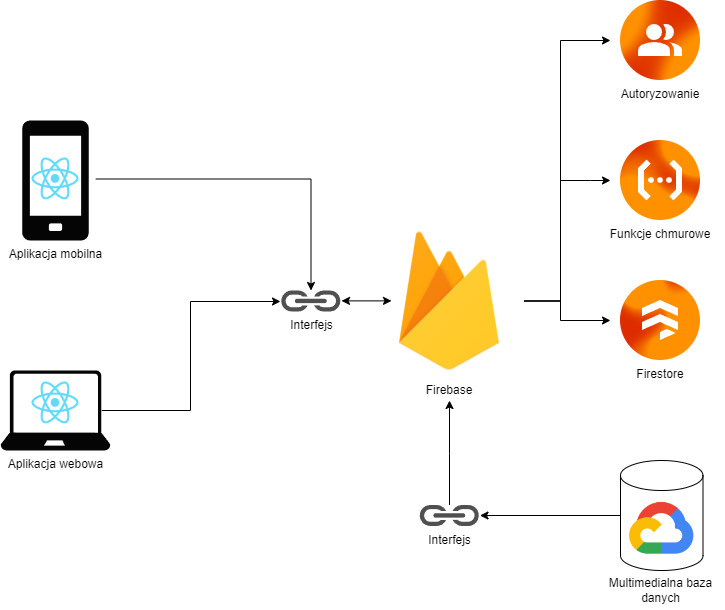
\includegraphics[width=\textwidth]{img/3/architektura.png}
        \caption{Schemat architektury systemu}
        \label{fig:architektura}
    \end{figure}

    \subsection{Stos technologiczny}
    Do wykonania projektu aplikacji, zostały wykorzystane następujące technologie:
    \begin{itemize}
        \item JavaScript,
        \item React,
        \item React Native,
        \item React Navigation,
        \item Expo,
        \item Firestore Database,
        \item Firebase Cloud Functions,
        \item Firebase Authentication,
        \item Google Storage,
    \end{itemize}

    \subsection{Środowisko programistyczne}
    Poszczególne warstwy aplikacji zostały stworzone przy użyciu zintegrowanego środowiska programistycznego (IDE). Mój wybór padł na WebStorm \cite{WebStorm}, gdyż jest on przystosowany do pracy z aplikacjami webowymi, oferuje integrację z systemem kontroli wersji i daje możliwość rozszerzenia edytora za pomocą pluginów. Środowisko to zostało stworzone na bazie IntelliJ IDEA udostępnianego przez JetBrains. \\
    
    Do pracy nad bazą danych, została użyta usługa Firestore Database \cite{Firestore}. Jest to dokumentowa baza danych w której wszystkie dane przechowywane są w formacie json. Jest to naturalny sposób przechowywania obiektów w JavaScript co pozwala na uproszczone przetwarzanie danych przez aplikację. Sam dokumentowy model danych jest prosty w użyciu jednak wymaga innego podejścia do organizacji danych. \\
    
    Użyte zostało także środowisko Android Studio \cite{AndroidStudio}. Jest to oficjalne narzędzie do tworzenia aplikacji mobilnych które zostało stworzone na bazie wcześniej wspomnianego IntelliJ IDEA. Pozwoliło mi to na skonfigurowanie wirtualnego urządzenia z wybraną wersją systemu Android (wersja 12) które następnie było przeze mnie wykorzystywane do testowania działania aplikacji. Android Studio jest dostępne bezpłatnie dla deweloperów i jest sugerowany przez Google jako domyślne rozwiązanie do tworzenia aplikacji mobilnych.

    \begin{figure}[H]
        \centering
        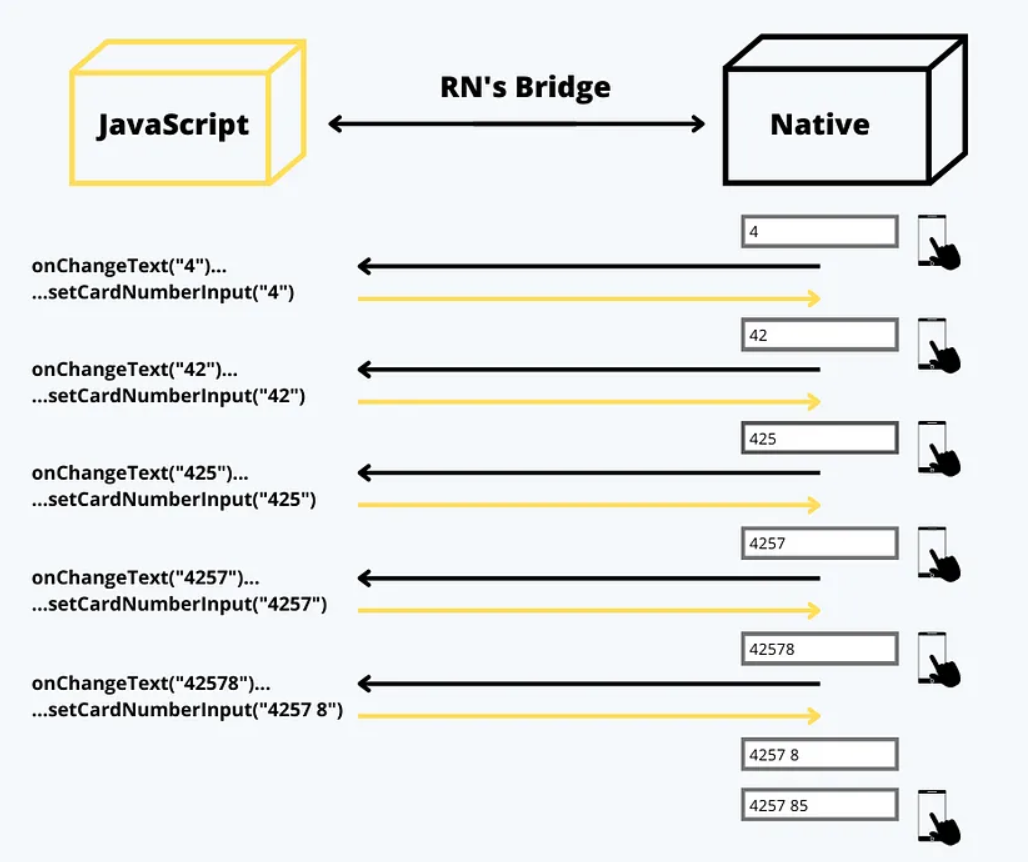
\includegraphics[width=0.8\textwidth]{img/3/react_native_concept.png}
        \caption{Sposób działania mostu w React Native, źródło: \textit{Jakub Kosmal, How does React Native work? Understanding the architecture}}
        \label{fig:react-native}
    \end{figure}
\newpage
\section{Projekt wstępny}
Aby zaprojektować graficzny interfejs użytkownika, wykorzystane zostało narzędzie Figma. Prezentacja makiety kilku ekranów aplikacji znajduje się pod \href{https://www.figma.com/proto/1yxKJbcj7I3atl6e7OpHO8/TravelApp?type=design&node-id=1-247&scaling=min-zoom&page-id=0%3A1&starting-point-node-id=1%3A154}{tym linkiem}.

W projekcie są pokazane przykładowe przejścia między wybranymi ekranami dostępnymi dla użytkownika. Warto wspomnieć że jest to jedynie makieta interfejsu która uległa znacznym zmianom względem wersji finalnej.

\subsection{Ekran logowania}
\begin{figure}[H]
    \centering
    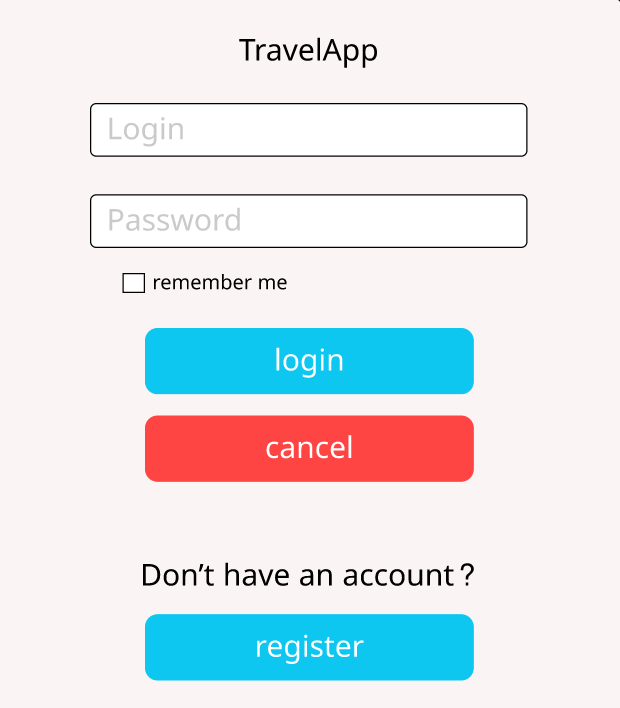
\includegraphics[width=0.5\textwidth]{img/4/logowanie.png}
    \caption{Ekran logowania do aplikacji}
    \label{fig:proj-wstepny-ekran-logowania}
\end{figure}

Na tym ekranie dostępne są dwa pola, do których użytkownik może podać swoje dane potrzebne w celu logowania się do aplikacji jeżeli posiada już konto. W przypadku kiedy konta nie posiada, może wybrać opcję pod przyciskiem "register" która spowoduje pojawienie się nowego ekranu. \\

\subsection{Ekran rejestracji}
\begin{figure}[H]
    \centering
    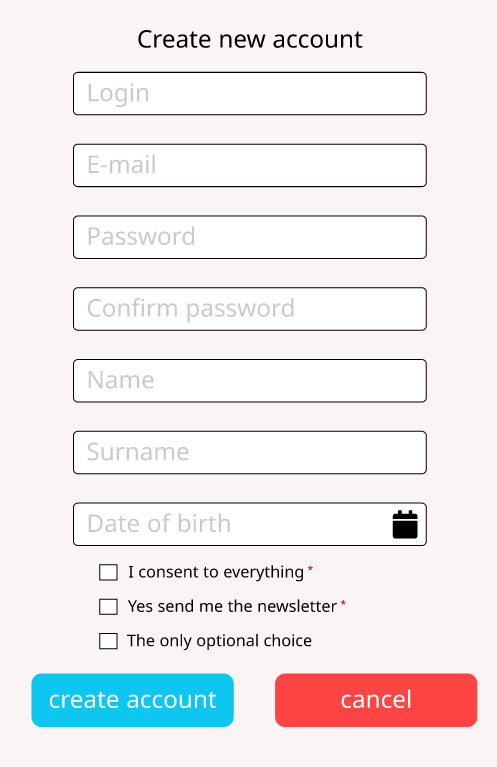
\includegraphics[width=0.5\textwidth]{img/4/rejestracja.png}
    \caption{Ekran rejestracji nowego użytkownika}
    \label{fig:proj-wstepny-ekran-rejestracji}
\end{figure}

Ekran rejestracji przedstawia formularz który użytkownik musi wypełnić w celu założenia nowego konta. Aby to zrobić, wymagane jest podanie loginu który będzie używany przez aplikację do rozpoznawania użytkowników wraz z adresem e-mail, hasłem oraz imieniem i nazwiskiem. Jako ostatnie pole wymagane jest podanie daty urodzenia.
Aby rejestracja mogła zostać ukończona, osoba zakładająca konto musi wyrazić odpowiednie zgody marketingowe i zaakceptować wysyłanie newslettera na podany wcześniej adres mailowy. Jeżeli wszystko zostanie podane, może on użyć przycisku "create account" aby dokończyć proces zakładania konta. W każdej chwili możliwa jest też rezygnacja i powrót do ekranu logowania poprzez wciśnięcie przycisku "cancel".

\subsection{Lista dostępnych atrakcji}
\begin{figure}[H]
    \centering
    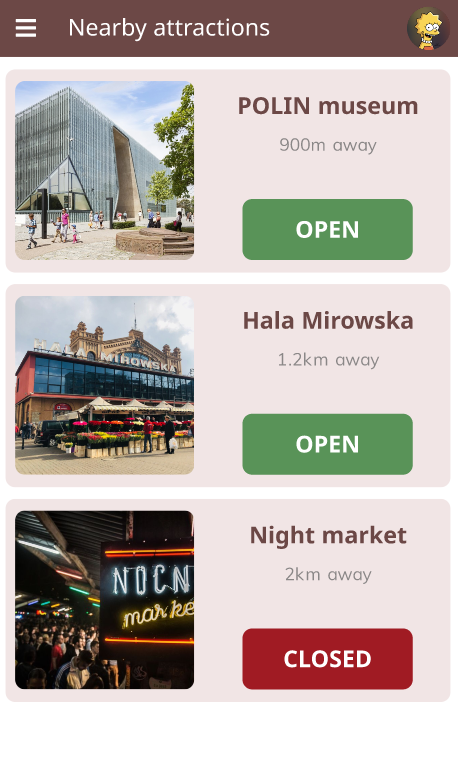
\includegraphics[width=0.5\textwidth]{img/4/lista.png}
    \caption{Ekran z listą dostępnych atrakcji turystycznych}
    \label{fig:proj-wstepny-lista}
\end{figure}

Na tym ekranie użytkownik ma dostępną listę dostępnych atrakcji które znajdują się w jego pobliżu. Lista obiektów posortowana jest względem jego bieżącej pozycji i ponadto podana jest informacja o tym, czy dana atrakcja jest w tej chwili możliwa do zwiedzenia poprzez komunikaty "OPEN" albo "CLOSED" wyświetlane w karcie każdej atrakcji. Podana jest również nazwa obiektu i zdjęcie przedstawiające atrakcję.
\newpage
\section{Implementacja}
\subsection{Schemat encji}
\newpage
\section{Testowanie}
\newpage
\section{Dalszy rozwój}
%W przypadku skończenia prac nad wersją na systemy Android, aplikacja może zostać rozszerzona na platformę iOS i na przeglądarki internetowe w postaci aplikacji webowej. \\
Planowane są również dodatkowe funkcjonalności aplikacji które nie zostały przewidziane do implementacji w ramach niniejszej pracy. Wśród nich znajdują się:
\begin{itemize}
    %\item oznaczanie atrakcji turystycznych do ulubionych przez użytkowników,
    \item ocenę danych obiektów przez użytkowników,
    \item dodanie placówek gastronomicznych,
    \item integrację z Google Maps,
    %\item pokazywanie dystansu do danego obiektu z poziomu aplikacji przy użyciu lokalizatorów GPS wbudowanych w urządzenia mobilne
\end{itemize}
\newpage
\section{Podsumowanie}

%--------------------------------------------
% Literatura
%--------------------------------------------
\cleardoublepage
\printbibliography

%--------------------------------------------
% Spisy (opcjonalne)
%--------------------------------------------
\newpage
\pagestyle{plain}

% Wykaz symboli i skrótów.
% Pamiętaj, żeby posortować symbole alfabetycznie
% we własnym zakresie. Ponieważ mało kto używa takiego wykazu,
% uznałem, że robienie automatycznie sortowanej listy
% na poziomie LaTeXa to za duży overkill.
% Makro \acronymlist generuje właściwy tytuł sekcji,
% w zależności od języka.
% Makro \acronym dodaje skrót/symbol do listy,
% zapewniając podstawowe formatowanie.
% //AB
% \vspace{0.8cm}
% \acronymlist
% \acronym{EiTI}{Wydział Elektroniki i Technik Informacyjnych}
% \acronym{PW}{Politechnika Warszawska}
% \acronym{WEIRD}{ang. \emph{Western, Educated, Industrialized, Rich and Democratic}}

\listoffigurestoc     % Spis rysunków.
\vspace{1cm}          % vertical space
% \listoftablestoc      % Spis tabel.
% \vspace{1cm}          % vertical space
% \listofappendicestoc  % Spis załączników

% Załączniki
% \newpage
% \appendix{Nazwa załącznika 1}

% \newpage
% \appendix{Nazwa załącznika 2}

\end{document}


